\section{Case Study}
\label{sec:case}

%%\wrm{Re-do case studies in Bud} \wrm{Break cart development down into
%%iterations} \wrm{How does the language naturally lead us to an order
%%independent style?  Talk about inserting all sorts of exotic stuff like queues
%%if we want a highly order-dependent imperative style.}

\begin{comment}

\jmh{We discussed the following on the phone.  (1) Handle shopping in two styles: destructive updates, and disorderly accumulation of increment/decrement.  (2) Do analysis on them to detect need for coordination in only the first, show that (annotated) 2PC removes the compiler warning.  (3) Deploy destructive+2PC on EC2 and show practical benefits of avoiding coordination.  (4) Evolve the program with new rules for checkout and/or inventory, show how the disorderly version is no longer monotonic.  Fix that  with 2PC where needed.  Also make sure the destructive version works with the new rules.  Now show that the disorderly version is still better than the destructive one, by coordinating only where needed.}

\jmh{Finally, show what would happen if you didn't coordinate the inventory bit, but tracked taint.  Note that tainted output is the stuff where programmers need to write compensation logic.}

\end{comment}

%%In this section, we implement two different styles of distributed shopping cart
%%applications in Bud.  First, we implement a ``destructive,'' overwriting
%%shopping cart application using a simple key-value store implemented in Bud.
%%Second, we implement a ``disorderly'' cart which accumulates updates in a 
%%set-wise fashion and describes how to combine the updates into a final result.

\jmh{Blah blah intro.}

We begin with a shopping cart built on a key-value store abstraction.  Each
cart is a pair \texttt{[key,value]}, where \texttt{key} is a unique session
identifier, and \texttt{value} is a Ruby array representing the set of items
contained in the cart at any time.  Addition and deletion actions to a cart
result in ``destructive'' overwrites, replacing the value associated with the
key with a new array reflecting the additions.  Deletion from an empty cart
\wrm{, as well as deletion of a non-existent element,} is ignored. 

Figure~\ref{fig:pdg-destructive} shows the Bloom code for this design.  The
\textbf{scratch} \texttt{kvstore} is defined by the KeyValueStore module (XXX
lines of Bloom not shown here), which the shopping cart extends via
inheritance.
%; it is used in a manner analogous to the \emph{put} function for hash tables.  
The set of shopping carts, represented by the persistent \textbf{table}
\texttt{bigtable}, is 
%kept  consistent across replicas
replicated by shipping \texttt{kvstore} tuples to other servers.
%%\jmh{Line numbers seem messed up.}

%We begin describing the logic from the outside \wrm{outside of what?}:

The client transmits \texttt{client\_action} tuples---corresponding to cart
updates---over the \texttt{action\_msg} \textbf{channel} to a server replica.
\jmh{which server replica?  all server replicas??} For each such arriving
tuple, line 2 probes \texttt{bigtable} to see if a record exists for the
session associated with the \texttt{action\_msg}.  If none is found (i.e., this
is the first update for a new session), then lines 2-6 generate an entry for
the new session in \texttt{bigtable}, appropriately initializing the array of
shopping cart contents.  Otherwise, the join conditions in lines 10-11 will be
satisfied, and lines 12-18 will instead be evaluated, ``replacing'' the array
at the next timestep with a new version.  Finally, when a server replica
receives a \texttt{checkout\_msg}, the array representing the cart contents in
\texttt{bigtable} associated with the given session is extracted (via the join
on lines 22-23) and sent back to the client.

Figure~\ref{fig:} shows an alternative shopping cart implementation, in which
updates are monotonically accumulated in a disorderly fashion and summarized
only at checkout.  Line 0 appends all client updates to the persistent table
\texttt{cart\_action}.  Lines 2-3 define \texttt{action\_cnt} as an aggregate
over \texttt{cart\_action}, in the style of an SQL group-by statement: for each
item associated with a cart, we separately count the number of times it was
added and the number of times it was deleted.  \jmh{what's up with lines 5-9?
initialize number of deletions to 0...to avoid failed join of additions with no
deletions, right?  Maybe less confusing to do another rule for status that
antijoins additions to deletions.  Or we could hack up an outerjoin syntax.}
\paa{I've frequently wanted an outerjoin syntax.  anti join? do you mean a
'subquery' with unlesss..include? ?} Lines 11-16 define the collection
\texttt{status} as a ternary join between the \texttt{checkout} message and two
copies of \texttt{action\_cnt} (one corresponding to additions and one to
deletions).  For each item, \texttt{status} contains its final quantity: the
difference between its number of additions and deletions (line 14).  The
replica then returns a \texttt{response} message to the client containing the
final quantity.  Because the disorderly implementation does not use a separate
storage system, it must explicitly replicate its state (lines 24-26).


\begin{figure}[t]
\begin{scriptsize}
\begin{verbatim}

0: kvstore <= action_msg.map do |a|
1:   if not bigtable.map{|b| b.key}.include? a.session
2:     if a.action == "Add"
3:       [a.server, a.client, a.session, a.reqid, [a.item]]
4:     elsif a.action == "Del"
5:       [a.server, a.client, a.session, a.reqid, []]
6:     end
7:   end
8: end
9: 
10: kvstore <= join([bigtable, action_msg]).map do |b, a|
11:   if b.key == a.session
12:     if a.action == "Add"
13:       [a.server, a.client, a.session, a.reqid, b.value.push(a.item)]
14:     elsif a.action == "Del"
15:       copy = b.value.clone;
16:       copy.delete_at(copy.index(a.item));
17:       [a.server, a.client, a.session, a.reqid, copy]
18:     end
19:   end
20: end
21:
22: response_msg <+ join([bigtable, checkout_msg]).map do |s, c|
23:   if s.key == c.session
24:     [c.client, c.server, s.key, s.value]
25:   end
26: end
27: 
28: action_msg <+ client_action.map{|a| a}


\end{verbatim}
\end{scriptsize}
\caption{Destructive Cart Implementation}
\label{fig:pdg-destructive}
\end{figure}

\begin{figure}[t]
\centering
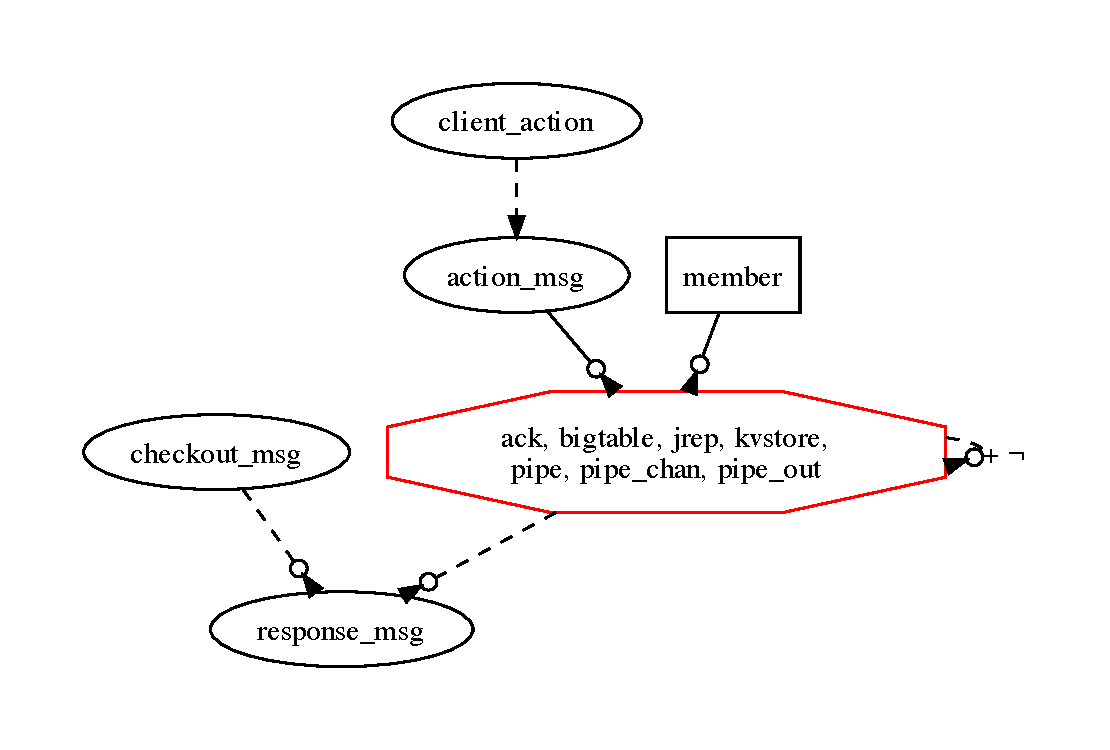
\includegraphics[width=0.9\linewidth]{fig/destructive.pdf}

\caption{Destructive Cart Analysis, with temporal cycles collapsed}
\label{fig:pdg-destructive-analysis}
\end{figure}


\subsection{Analysis}


For each cart, we apply whole-program analysis techniques to discover points of 
order.  The Bud interpreter automatically generates
a graphical representation of the dependency graph of collections through rules,
(and hence the 
flow of tuples) as a staged dataflow.  Each node in the graph is either
a collection or a cluster of collections (as described below).  A directed edge from node $A$ to node $B$ captures the fact that $B$ is in the lhs of a Bloom statement with $R$ in the rhs (or in a join expression in the rhs).  Edges are annotated based on the operators and lhs types in the rules.  Rules that involve synchronous timesteps---i.e. a \texttt{$<$+} operator with a {\bf table} lhs---are marked with a $+$.  Rules that involve asynchronous messaging---i.e., a \texttt{$<+$} operators with a {\bf channel lhs}---are indicated by a dashed line.  Nonmonotonic rhs predicates result in edges marked with a $\lnot$.  Strongly connected components having both a $\lnot$ and a $+$ edge are grouped into ``temporal clusters'', 
%%\jmh{capturing what? the fact that they must recurse over multiple timesteps?}
collapsing the mutually dependent collections into a single node.  All edges
incident to a temporal cluster, including the self-edge, are points of order,
as are any negated edges.
%%Individual monotonic components 
%%(or strata) are surrounded by a dotted rectangle.  A point of order occurs
%%wherever an edge crosses strata, or at any self-edge attached to a temporal cluster.
Points of order are indicated by lightning bolts.

To resolve a point of order, the programmer may add coordination logic, which typically ensures  ordered delivered tuples, and/or guarantees that a boundary condition has been irrevocably crossed (e.g., there will be no more tuples).
% Instead of reanalyzing the augmented program, we associate coordination code
% with an annotation that can
% be interpreted as a contract about a point of order.  Such contracts will
% typically guarantee an ordering over arriving tuples, or guarantee a 
% a barrier-passing condition (e.g., indicating that there will be no more tuples).

\jmh{the subsequent discussion should be pared down and made simple.  updates are non-monotonic.  we see it in the points of order.  If we resolve using coordination a la 2PC, we get a round of coord for every client action.  This is the kind of thing Amazon didn't like for availability.  However, if we examine the disorderly figure, we see that the point of order is at checkout only, which is what Amazon wanted.}
%%Intuitively, the ``destructive'' cart based on
%%array mutation should be non-monotonic due to the transience of its state; this should make it sensitive to the order
%%of its inputs.
Although there is no syntactically obvious non-monotonicity in the destructive
cart code as shown, the underlying key-value store uses the \texttt{$<$-} operator to model updateable state, which results in non-monotonicity.\footnote{Our full-length paper expands the SCC to analyze the
key-value store in detail.}
The global analysis shown in Figure~\ref{fig:pdf-destructive}
indicates that there are
points of order between \texttt{action\_msg} and the temporal cluster,
and between the temporal cluster and itself.
%%This means that the arrival 
%%timing and ordering of both client updates (via \texttt{iaction}) and
%%server replication (via the meta-edge in the temporal cycle from 
%%\texttt{kvstore} to itself) may affect the
%%end results.  
To ensure a consistent final state across all replicas, we may require coordination
between client and server at every update to the cart, and between the 
server and all replicas at each update.   

%%We can easily achieve coordination without modifying the cart implementation
%%by redefining the key-value store to extend
%%a reliable or quorum-based delivery module instead of the best-effort module
%%that the basic key-value store extends, and require acknowledgement from a server or a %%quorum of servers, respectively.
%%The simplest (and least performant) approach is to require unanimous quorum,
%%approximating ``eager replication''~\cite{dangers} via two-phase commit.
A programmer could resolve this point of order by adapting the key-value store
to require reliable delivery to all replicas before acknowledging a client update, by
making the key-value store inherit from a superclass providing a reliable delivery
abstraction (6 LOC).
Such ``eager replication''~\cite{dangers} would incur a cost of a round of messages
per server per client update, and substantially decrease system throughput.  
Because we only care about the set of elements contained in the value array
and not its order, we might be tempted to argue that 
the shopping cart application is eventually consistent
when asynchronously updated, and forego the synchronization.  Unfortunately, such informal reasoning can hide serious bugs: consider what happens if a delete update is received
before the addition it was intended to cancel.



\begin{figure}[t]
\begin{scriptsize}
\begin{verbatim}
0:  cart_action <= action_msg.map { |c| [c.session, c.item, c.action, c.reqid] }
1:
2:  action_cnt <= cart_action.group([cart_action.session, 
3:    cart_action.item, cart_action.action], count(cart_action.reqid))
4:
5:  action_cnt <= cart_action.map do |a| 
6:    unless cart_action.map{|c| [c.session, c.item] if c.action == "D"}.include? [a.session, a.item] 
7:      [a.session, a.item, 'D', 0]
8:    end 
9:  end
10: 
11: status <= join([action_cnt, action_cnt, checkout]).map do |a1, a2, c| 
12:   if a1.session == a2.session and a1.item == a2.item 
13:   and a1.session == c.session and a1.action == "A" and a2.action == "D"
14:     [a1.session, a1.item, a1.cnt - a2.cnt] if (a1.cnt - a2.cnt) > 0
15:   end
16: end
17:
18: response_msg <= join([status, checkout]).map do |s, c| 
19:   if s.session == c.session
20:     [c.client, c.server, s.session, s.item, s.cnt]
21:   end
22: end
23: 
24: action_msg <+ join([action_msg, member]).map do |a, m|
25:   [m.player, a.server, a.session, a.item, a.action, a.reqid]
26: end
27: 
28: checkout_msg <+ join([checkout_msg, member}).map do |c, m|
29:   [m.player, c.server, c.session, c.reqid]
30: end


\end{verbatim}
\end{scriptsize}
\caption{Disorderly Cart Implementation}
\label{fig:pdg-disorderly}
\end{figure}

\begin{figure}[t]
\centering
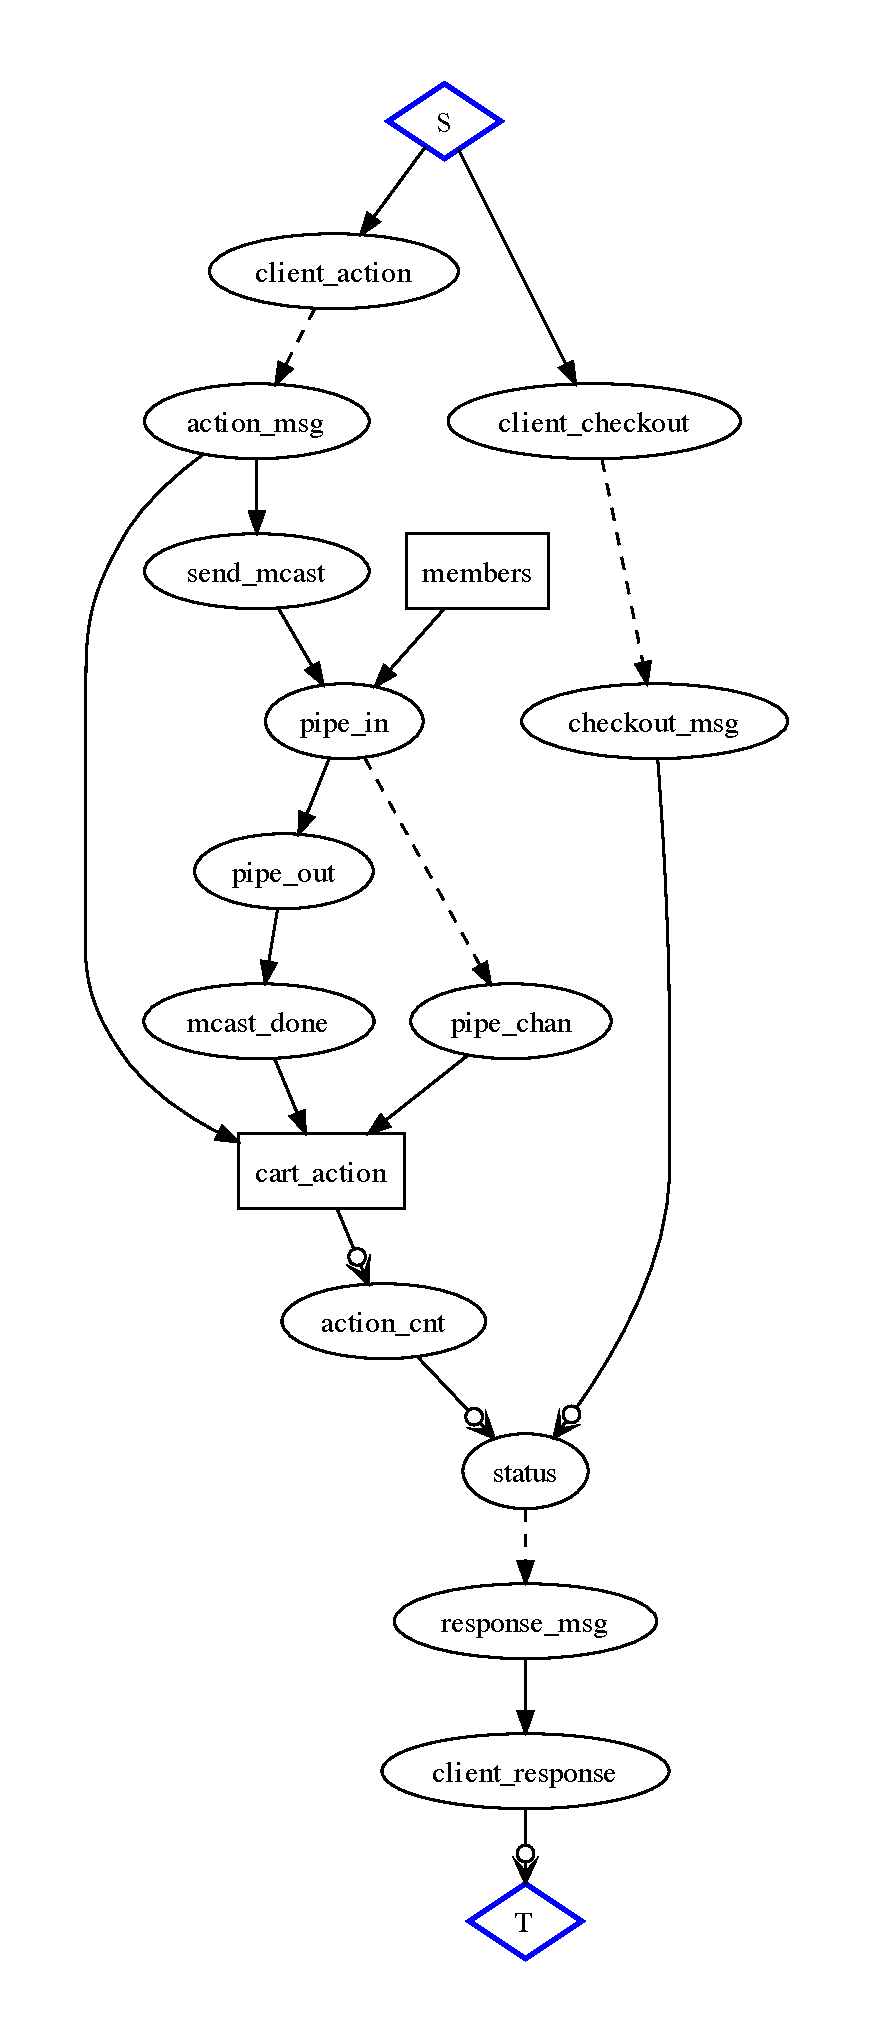
\includegraphics[width=0.7\linewidth]{fig/disorderly.pdf}
\caption{Disorderly Cart Analysis}
\label{fig:pdg-disorderly-analysis}
\end{figure}




Turning our attention to the disorderly figure,
\begin{comment}
 shows dotted lines indicating that 
\texttt{action\_msg} (owned by the server) is derived from \texttt{client\_action} 
(owned by the client) via an asynchronous message, and that \texttt{action\_msg} 
derives itself via messages when it is replicated.  However, the analysis
shows that because these derivations are strictly monotonic, no points of
order are crossed.  Hence, clients may send and servers may replicate 
updates without any coordination: regardless of timing and ordering, the end
result will be the same.

The analysis does indicate a point of order at checkout, when a \texttt{checkout}
message is joined with an aggregate over the set of updates.  While the 
accumulation of state has been monotonic, summarization of the cart state
requires us to assume (or prove) that there will be no further updates.
Consider a checkout message and a final update message racing from a client
to one of the replicas: the order in which they arrive will surely affect
the contents of the response message.  
\end{comment}
we see that communication (via \texttt{action\_msg}) between client and server
and between servers and replicas crosses no points of order, so all such
communication will converge to the same final state without coordination.
There is, however, a point of order at checkout, when a \texttt{checkout}
message is joined with an aggregate over the set of updates.  While the 
accumulation of state has been monotonic, summarization of the cart state
requires us to assume (or prove) that there will be no further updates.
Consider a checkout message and a final update message racing from a client
to one of the replicas: the order in which they arrive will surely affect
the contents of the response message.  
We need only coordinate once per session to
ensure that the response to the client is deterministic.

Like embarrassing parallelism in parallel computing, strictly monotonic programs
are rare in the distributed systems domain.  In this running example we studied
two candidate implementations of a simple distributed application with the aid of
our tool, and discovered that both have points of order.  Deciding that the disorderly
approach is ``better'' required us to apply domain knowledge: checkout happens
once per session, and is a more efficient coordination point than state update and replication, 
which occur repeatedly -- this is not unlike synchronizing on read rather than write 
in write-dominant systems generally.  Our analysis assisted us by highlighting the few locations where program correctness may depend upon costly synchronization, which may
result in decreased throughput and availability.  

\jmh{Challenge text that was kicking around and needs to be addressed here: we don't really say how we discourage a programmer from a destructive implementation, or help them migrate from that implementation to a better one.  Ideally we'd find ways to ``push back'' coordination requirements to local nodes and/or points of the program that don't have latency constraints.}

